\section{Source of Systematics}
In this section, we will discuss the possible sources of systematics that could affect the covariance matrix. 

\subsection{Box Replication Effect}\label{sec:boxreplication}
The box replication effect arises from replication of the simulation box in order to increase the volume of the simulation. In our setup, patches around special directions suffer the most from the box replication effect. To roughly assess the effect, we can compare the covariance matrices made from the patches of those directions and the rest of the patches.

Here, we defined the directions where are suspected to be affected by the box replication effect by the following criteria:
\begin{itemize}
    \item data points around equator: $ \left| \theta_i - \frac{\pi}{2} \right| \leq R_{\text{patch}} $
    \item data points around the edges of octant: $ \left| \phi_i - \frac{k\pi}{2} \right| \leq R_{\text{patch}} $ for $k=0,1,2,3$
\end{itemize}
where $(\theta_i, \phi_i)$ denotes the center of the patch $i$, and $R_{\text{patch}} = 5\sqrt{2}\, \mathrm{\deg}$ is the half diagonal length of the patch. 

We found that the patches including the point $(\theta_i, \phi_i) = (\pi/2, 0)$ have a signnificantly variated mean and variance, even comapared to the rest of suspects. Therefore, we simply discarded this point as it will bias the result. 

Finally, we obtain $70$ patches from each realization, and $1400$ patches for TILED simulations and $770$ patches for BIGBOX simulations in total.

Figure~\ref{fig:boxreplication_ell_cov} and Figure~\ref{fig:boxreplication_nu_cov} show the average ratios of the covariance matrices and correlation matrices between BIGBOX and TILED simulations. Regardless the noisy behavior of bispectrum, the ratio are much closer to unity for the suspected patches. This implies that the box replication effect is significantly enhance the covariance matrix.

\begin{figure}[ht]
    \centering
    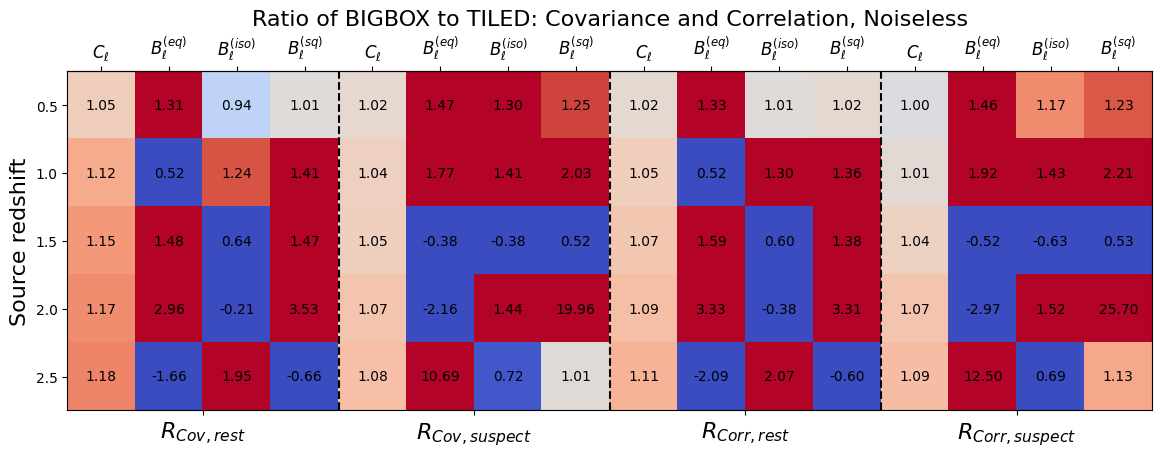
\includegraphics[width=0.7\textwidth]{figures/BR/BR_ratio_ell_cov.png}
    \caption{The ratios of covariance matrices and correlation matrices of power spectrum and bispectrum between the patches around special directions and the rest of the patches. }
    \label{fig:boxreplication_ell_cov}
    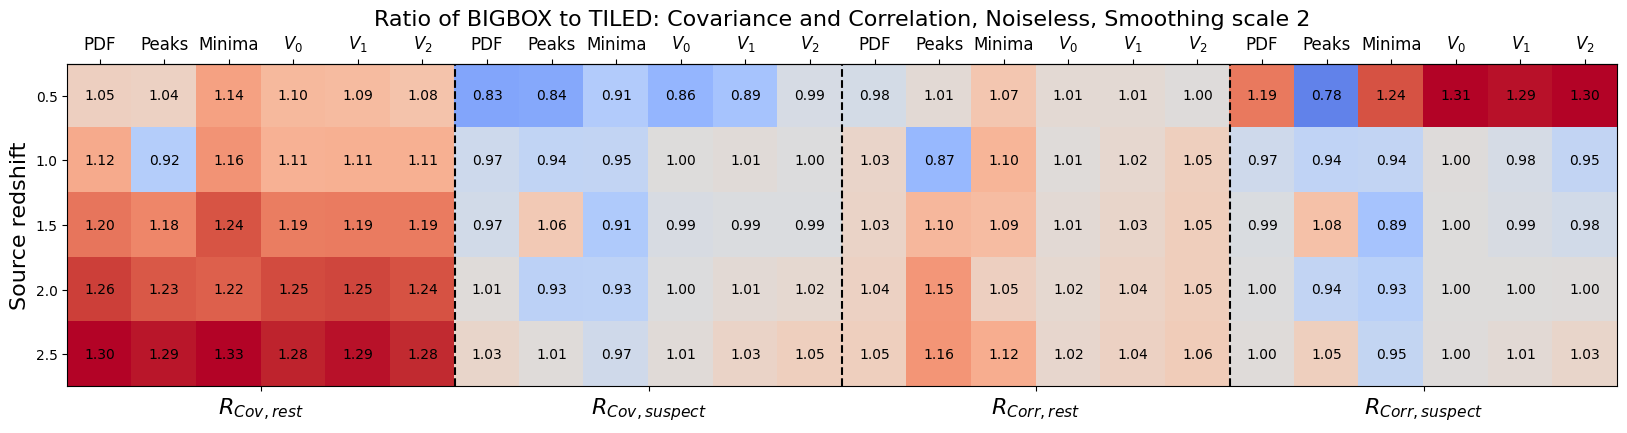
\includegraphics[width=\textwidth]{figures/BR/BR_ratio_nu_cov.png}
    \caption{The same as Figure~\ref{fig:boxreplication_ell_cov}, but for PDF, peak/minima counts and Minkowski functionals. The box replication effect significantly enhances the covariance matrix.}
    \label{fig:boxreplication_nu_cov}
\end{figure}

Figure~\ref{fig:boxreplication_ell} and~\ref{fig:boxreplication_nu} show the comparison of the ratios of mean and variance of each Statistics. Clearly, the suspected patches have biased mean values. The variance ratios are closer to unity, which means that the variance of the suspected patches is larger than the rest of the patches.

\begin{figure}[p]
    \centering
    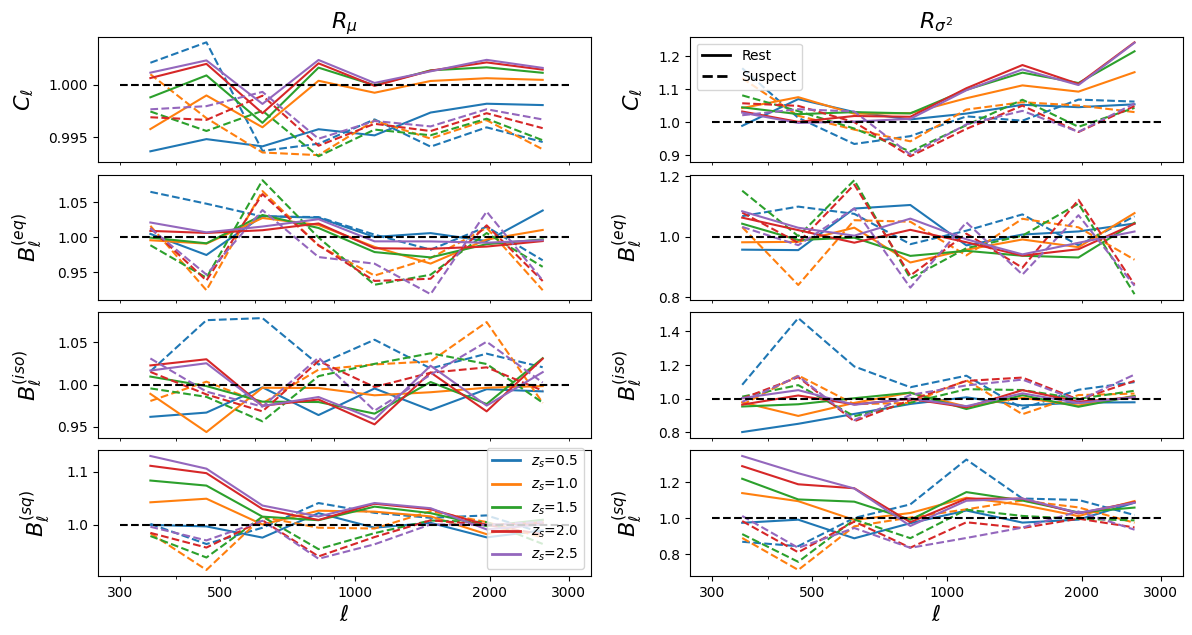
\includegraphics[width=0.9\textwidth]{figures/BR/BR_ratio_ell.png}
    \caption{The ratios of mean and variance of power spectrum and bispectrum between the patches around special directions and the rest of the patches. The mean of suspected patches are biased and the variance is larger.}
    \label{fig:boxreplication_ell}
    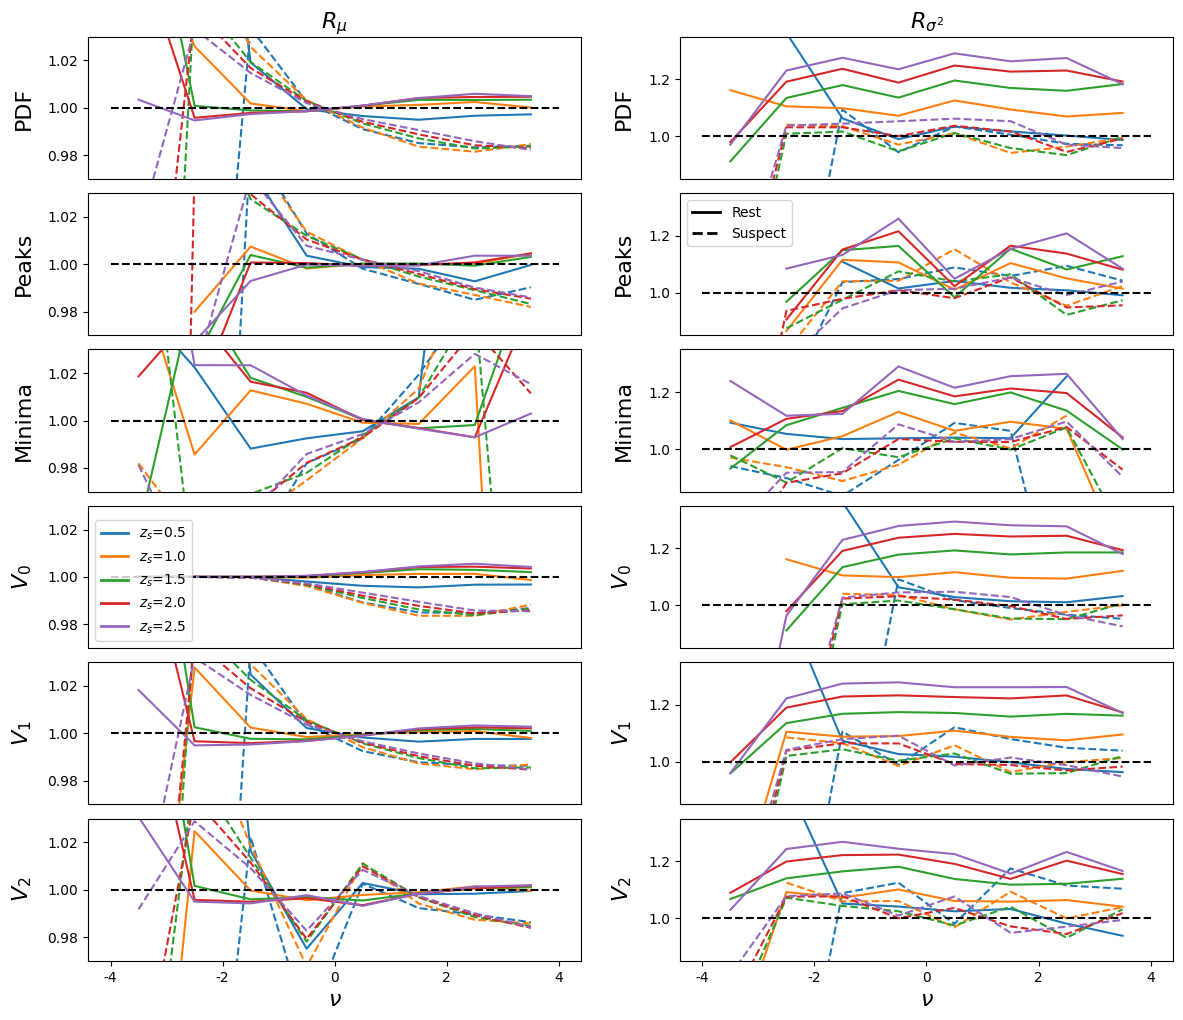
\includegraphics[width=0.9\textwidth]{figures/BR/BR_ratio_nu.png}
    \caption{The same as Figure~\ref{fig:boxreplication_ell}, but for PDF, peak/minima counts and Minkowski functionals. The suspected patches tend to have more extreme values and larger variance.}
    \label{fig:boxreplication_nu}
\end{figure}

\section{flat-sky vs. full-sky}
The flat-sky approximation is a good approximation for small patches on the sky. However, the flat-sky approximation breaks down for large patches. In this section, we conduct a test for angular power spectrum, PDF, and peak/minima counts to see how the flat-sky approximation affects the statistics.